\begin{figure}[t!]
\centering
\footnotesize
\begin{tabular}{@{}c@{\;}c@{\;}c@{\;}c@{}}
& Samples & Power spectrum & Radial mean \\
%
%=====================
%
\rotatebox{90}{\qquad Poisson Disk} & 
\begin{tikzpicture}
  \node[anchor=south west,inner sep=0] (image) at (0,0)
  {
    \pdfliteral{ 1 w}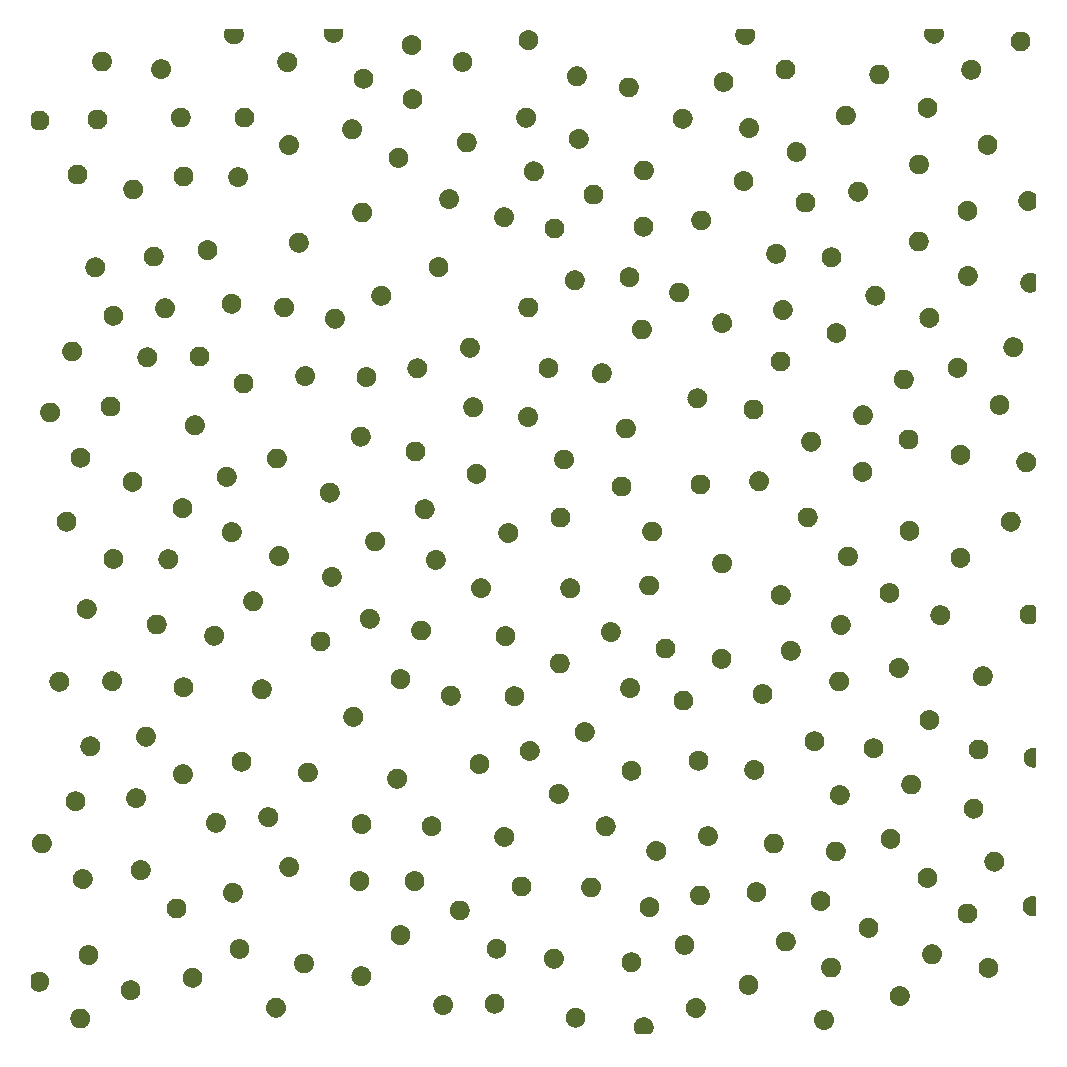
\includegraphics[width=1.4in,page=1]{pointset/points-dartthrowing-n256.pdf}
  };

  \begin{scope}[x={(image.south east)},y={(image.north west)}]
  \draw[black,thick] (0,0) rectangle (1,1);
  \end{scope}
\end{tikzpicture} 
&
\begin{tikzpicture}
  \node[anchor=south west,inner sep=0] (image) at (0,0)
  {
    \pdfliteral{ 1 w}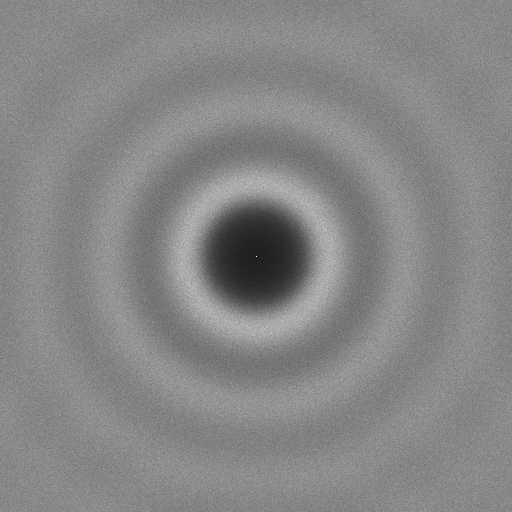
\includegraphics[width=1.4in,page=1]{power-spectra/powerspectrum-dartthrowing-n4096.png}
  };

  \begin{scope}[x={(image.south east)},y={(image.north west)}]
  \draw[black,thick] (0,0) rectangle (1,1);
  \end{scope}
\end{tikzpicture}
&
\begin{tikzpicture}
  \node[anchor=south west,inner sep=0] (image) at (0,0)
  {
    \pdfliteral{ 1 w}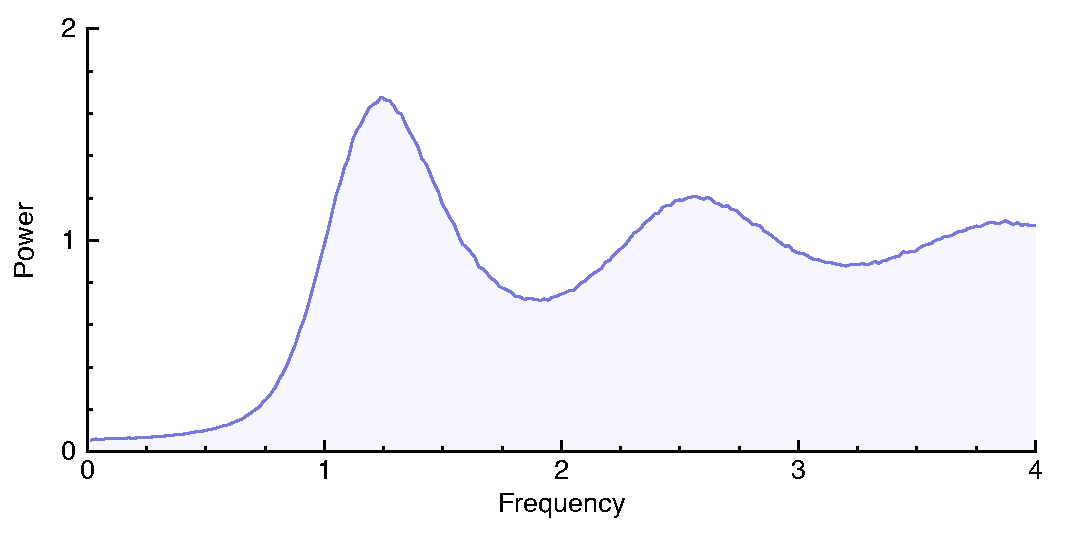
\includegraphics[width=2.8in,page=1]{power-spectra/radial-mean-dartthrowing-n4096.pdf}
  };

  \begin{scope}[x={(image.south east)},y={(image.north west)}]
  \draw[black,thick] (0,0) rectangle (1,1);
  \end{scope}
\end{tikzpicture}
\\
%
%=====================
%
\rotatebox{90}{\qquad\quad CCVT} & 
\begin{tikzpicture}
  \node[anchor=south west,inner sep=0] (image) at (0,0)
  {
    \pdfliteral{ 1 w}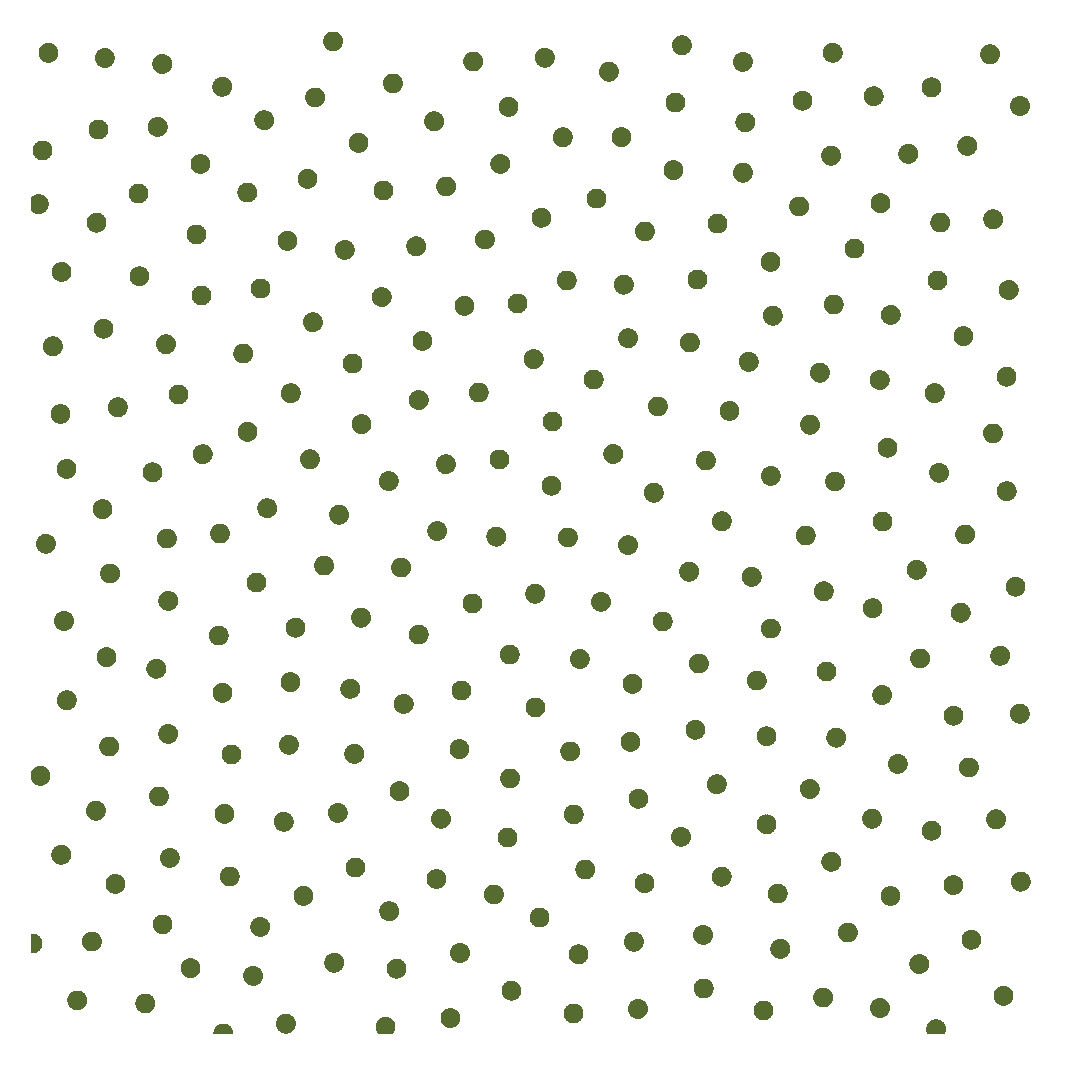
\includegraphics[width=1.4in,page=1]{pointset/points-ccvt-n256.pdf}
  };

  \begin{scope}[x={(image.south east)},y={(image.north west)}]
  \draw[black,thick] (0,0) rectangle (1,1);
  \end{scope}
\end{tikzpicture} 
&
\begin{tikzpicture}
  \node[anchor=south west,inner sep=0] (image) at (0,0)
  {
    \pdfliteral{ 1 w}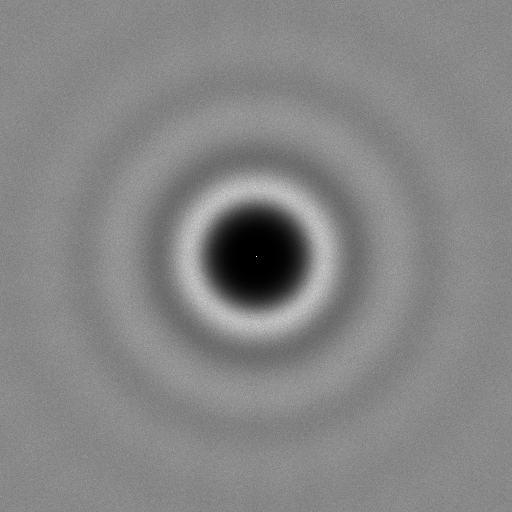
\includegraphics[width=1.4in,page=1]{power-spectra/powerspectrum-ccvt-n4096.png}
  };

  \begin{scope}[x={(image.south east)},y={(image.north west)}]
  \draw[black,thick] (0,0) rectangle (1,1);
  \end{scope}
\end{tikzpicture}
&
\begin{tikzpicture}
  \node[anchor=south west,inner sep=0] (image) at (0,0)
  {
    \pdfliteral{ 1 w}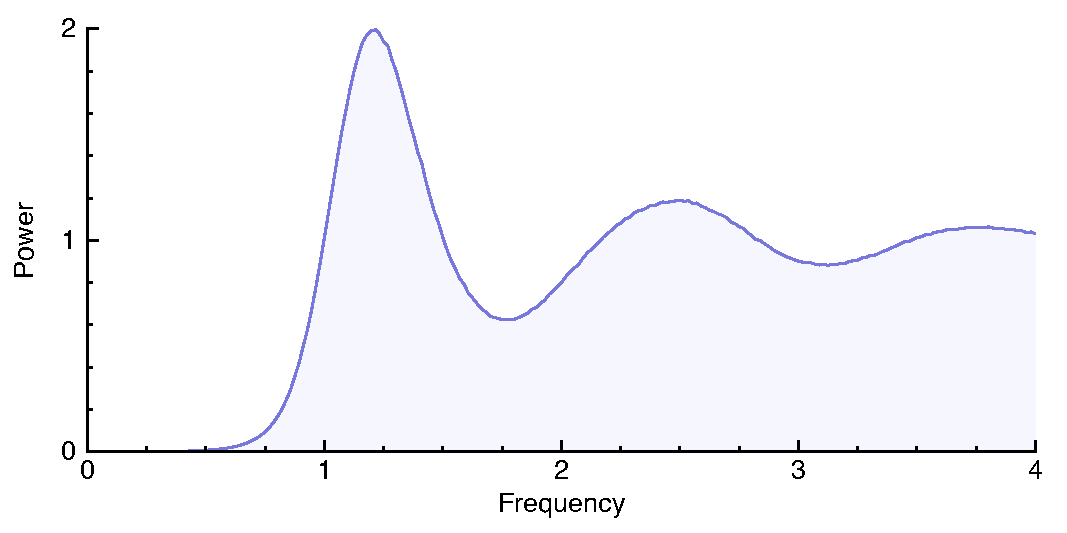
\includegraphics[width=2.8in,page=1]{power-spectra/radial-mean-ccvt-n4096.pdf}
  };

  \begin{scope}[x={(image.south east)},y={(image.north west)}]
  \draw[black,thick] (0,0) rectangle (1,1);
  \end{scope}
\end{tikzpicture}
\end{tabular}
%
\caption{\label{fig:powspec-radialmean-bluenoise}%
Illustration of some well known blue noise samplers with the corresponding Fourier expected power spectra and the corresponding radial mean of their expected power spectra.}
\end{figure}